\documentclass{beamer}
\usepackage[latin1]{inputenc}
\usepackage{amsmath}
\usepackage{graphicx}
\usepackage{multimedia}
\usepackage{caption}
\usetheme{default}
\usecolortheme{default}
\definecolor{darkred}{RGB}{24,0,0}
\setbeamercolor{title}{fg=red}
%\setbeamercolor{frametitle}{fg=black}
\setbeamertemplate{blocks}[rounded][shadow=true]
\setbeamertemplate{itemize items}[square]
\usefonttheme{serif}
\title{\textit{\textbf{\'Atomo de Hidrogeno relativista en el formalismo de Dirac.}}}
\author{Juan Nicol\'as Garavito Camargo \\ Juan David Orjuela Zu\~niga}
\institute{Universidad de los Andes, Bogot\'a, Colombia}
\date{May 27, 2015}
\begin{document}

\begin{frame}
\titlepage
\author
\institute
\begin{figure}
%\rule{1.28cm}{0.72cm}

\includegraphics[scale=0.35]{Figures/logo.png}
\end{figure}
\end{frame}


\begin{frame}
\begin{equation}
i\hbar\frac{\partial}{\partial t} \psi (\vec{r}, t)=-\frac{\hbar^2}{2m}\nabla^2  \psi (\vec{r}, t) + V(\vec{r}) \psi (\vec{r}, t)
\end{equation}

\begin{equation}
\left( \nabla^2 - \dfrac{1}{c^2}\dfrac{\partial^2}{\partial t^2} - \dfrac{m^2c^2}{\hbar^2}   \right)\psi(\mathbf{r}, t) = 0
\end{equation}
\end{frame}

\begin{frame}
\begin{figure}
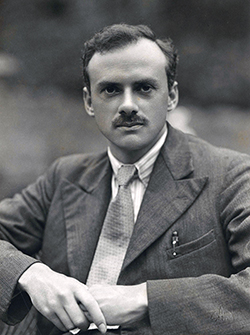
\includegraphics[sclae=0.5]{Figures/dirac.jpg}
\end{figure}
\end{frame}

\begin{frame}
\begin{equation}
\dfrac{1}{c}\dfrac{\partial \psi_i(\mathbf{r},t)}{\partial t} =
- \sum \limits_{k=x,y,z} \sum \limits_{n=1}^{N}\alpha^k_{i,n} \dfrac{\partial \psi_n}{\partial k} -
\dfrac{imc}{\hbar}\sum \limits_{n=1}^{N}\beta_{i,n}\psi_n(\mathbf{r}, t)
\end{equation}
\end{frame}

\begin{frame}
\begin{equation}
E\phi(\mathbf{r},t) =
(c\widetilde{\alpha}\cdot \hat{\mathbf{p}} + \widetilde{\beta}mc^2 + V(r))\phi(\mathbf{r})
\end{equation}

\begin{equation}
\widetilde{\alpha_i}=
\begin{pmatrix}
0 & \widetilde{\sigma}_i\\
\widetilde{\sigma}_i & 0 \\
\end{pmatrix}
\end{equation}

\begin{equation}
\widetilde{\beta}=
\begin{pmatrix}
\widetilde{\mathbf{I}}_2 & 0\\
0 & -\widetilde{\mathbf{I}}_2 \\
\end{pmatrix}
\end{equation}

\end{frame}

\begin{frame}
Para el \'atomo de Hidr\'ogeno se debe solucionar (\ref{dirac})
con un potencial $V(r)$ definido como:

\begin{equation}
V(r) = \dfrac{Ze^2}{4\pi\epsilon_0 r^2}
\end{equation}

La ecuaci\'on de Dir\'ac para este potencial se expresa como:

\begin{equation}\label{eq:diracvr}
(c \widetilde{\alpha} \cdot \hat{p} + \widetilde{\beta} m c^2 + V(r) ) \phi(r) = E \phi (r)
\end{equation}
\end{frame}

\begin{frame}
\begin{equation}\label{eq:alphap}
\widetilde{\alpha} \cdot \hat{\mathbf{p}} = -i \hbar \widetilde{\alpha} \cdot \nabla
\end{equation}

\begin{equation}\label{eq:nabla}
\mathbf{\nabla} =  \hat{\mathbf{r}}(\dfrac{\partial}{\partial r}) - \dfrac{i}{\hbar}\dfrac{\hat{\mathbf{r}}}{r} \times \mathbf{L}
\end{equation}

Por lo tanto (\ref{eq:alphap}) se puede escribir en t\'erminos de (\ref{eq:nabla}) como:

\begin{equation}\label{eq:alphap2}
\widetilde{\alpha}\cdot \mathbf{\hat{p}} = -i\hbar \widetilde({\alpha}\cdot \hat{\mathbf{r}}(\dfrac{\partial}{\partial r}) - 
\dfrac{i}{\hbar}\widetilde{\alpha}\cdot \dfrac{\hat{\mathbf{r}}}{r} \times \mathbf{L})
\end{equation}
\end{frame}

\begin{frame}{N\'umero cuantico $\kappa$}
\begin{equation}
\widetilde{\hat{K}} = \widetilde{\hat{L}}\cdot \widetilde{\sigma} + \hbar
\end{equation}

Con autovalor $-\hbar \kappa$ y donde $\kappa$ puede tomar los siguientes
valores:

\[ \kappa = 
\begin{cases}
-l - 1 \rightarrow j = l + 1/2  \\
l \rightarrow j = l - 1/2 \\ 
\end{cases}
\]  

\end{frame}

\end{document}
